\section{Architecture}

\begin{figure}[H]
  \centering
    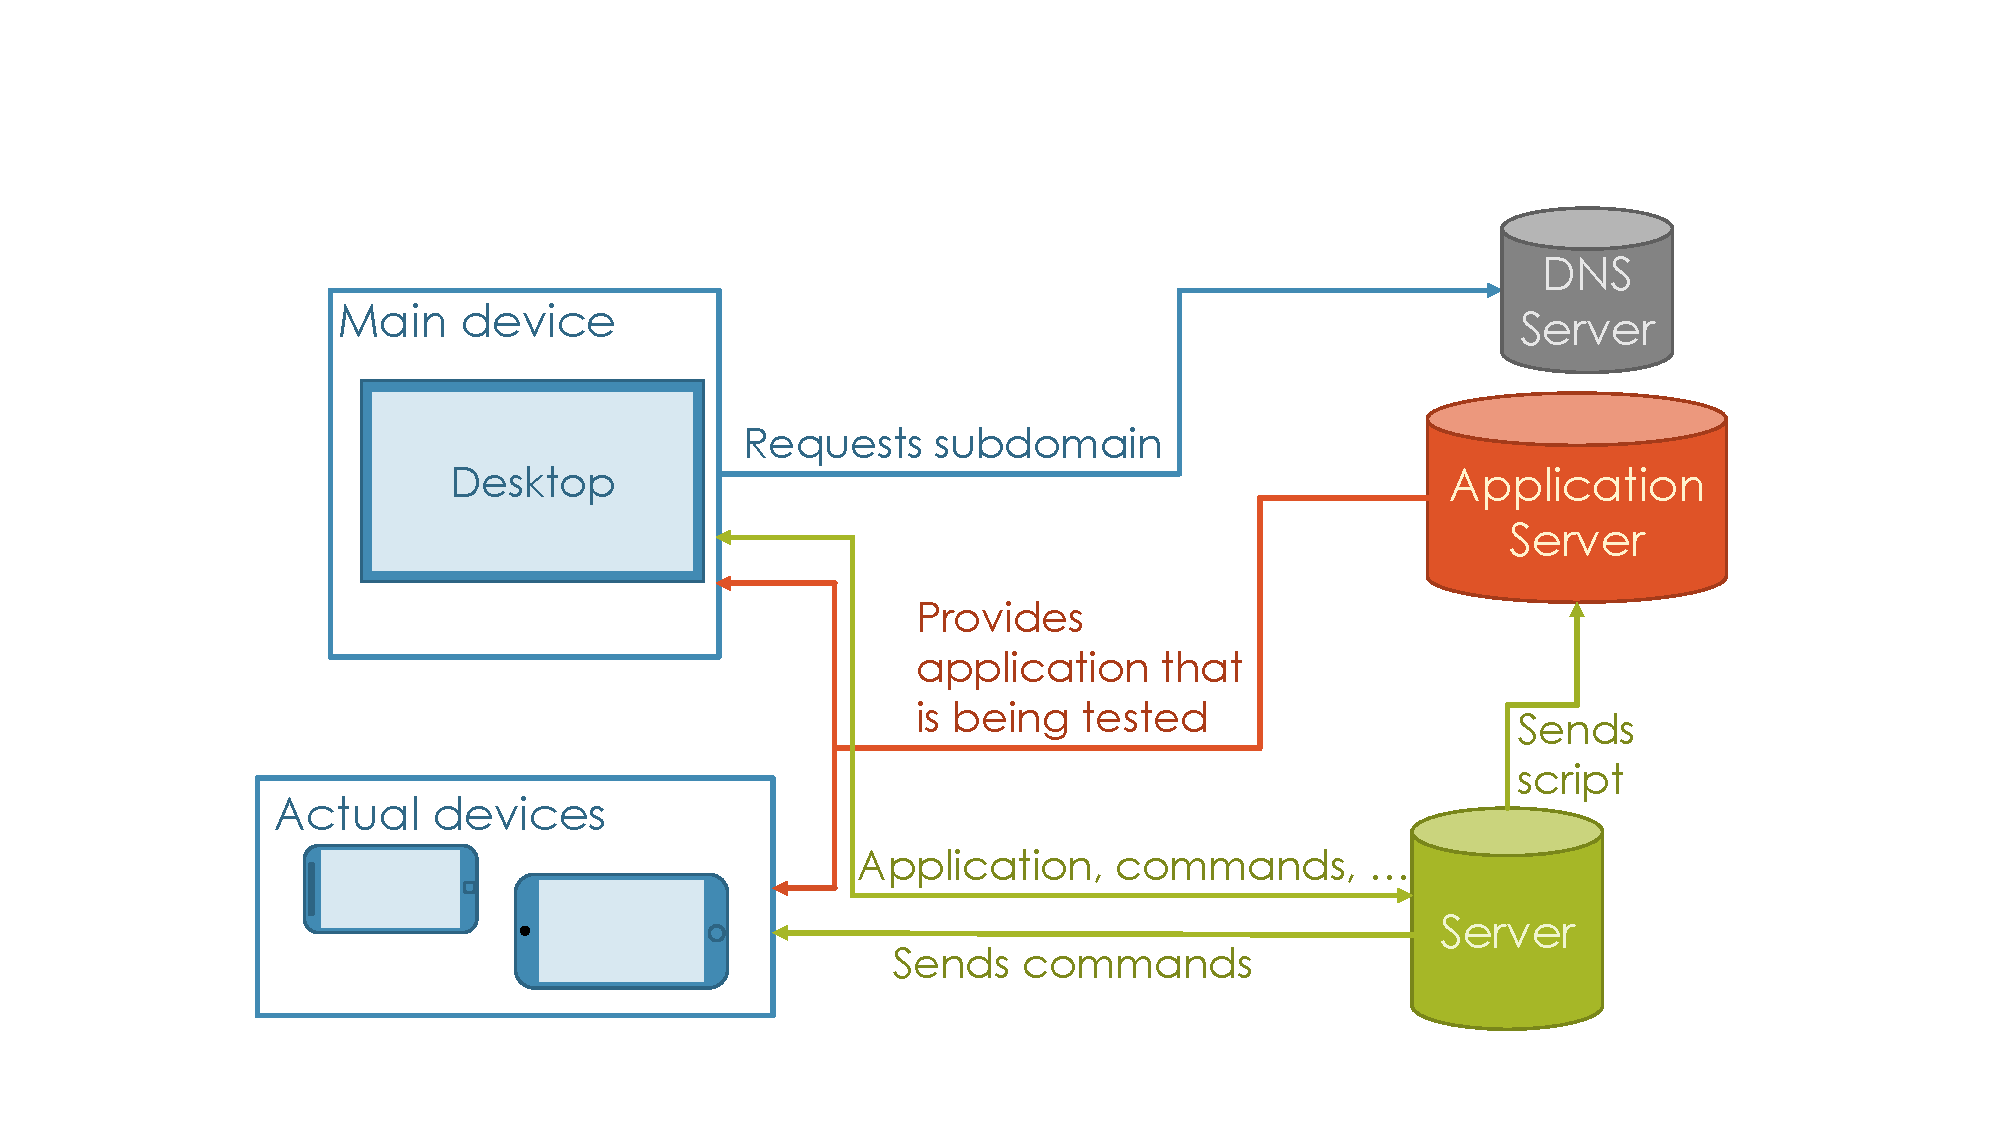
\includegraphics[width=1.0\textwidth]{images/architecture.pdf}
	\caption{Architecture of our tools}
	\label{fig:architecture}
\end{figure}

\section{Choice of Technologies}

HTML5, CSS3, local storage, ...

\subsection{node.js}

\subsubsection{Express}

\subsubsection{shortid}

\subsection{rainbow-dns}

\subsection{JavaScript Libraries and CSS Frameworks}

\subsubsection{Socket.io}

\subsubsection{Bootstrap}

\subsubsection{jQuery}

\subsubsection{jQuery UI}

\subsubsection{jQuery.qrcode}

\section{General Features}
Script inside cross-device applications for receiving and excuting commands

\section{Device Emulation}

Devices emulated as iframes
Only resolution emulated
Settings menu that can be collapsed and extended

Browser state: DNS server, URL based on ID of the device, unknown URLs forwarded to usual DNS server

Device scaling: CSS property "transform"

\section{Connecting Real Devices}

QR code that contains URL of our system

\section{Shared JavaScript Console}

eval used inside script

\section{Function Debugging}

overwriting of debugged functions to determine device where the function is called
when the debugging is started, the original function is stored and overwritten by a function that highlights the device, then calls the original function, then unhighlights the device
when the user does not debug a function anymore, the original function is restored
debug in the extension called with original function

Chrome Extension

HTML inspection

\section{Shared CSS Editor}

Stylesheet added in the script inside the application
Rules inserted into stylesheet

\section{Record/Replay}

Recording:
Event handlers are assigned as soon as page is loaded so no-one else can add event handlers earlier, but events only recorded when recording is enabled
Capturing event handlers on document --> no one can receive events first and modify the page or stop the event from propagating
After recording, event sequences are sent to the server, removal of circular structures before sending events

Determining the target of an event: When the event is recorded, the path through the document to the target element is recorded
If an ID is encountered, all parent elements are not required for finding the target element
--> Move up from the target element until the first ID is encountered
Consider Shadow DOM for event hierarchy

Replaying:
Events are triggered using setTimeout
TextEvent in addition to KeyEvent for replaying text input
Manually setting scrolling position for replaying scrolling
Manually checking if key pressed is backspace and manually erase char before caret
Before replaying event sequences and list of breakpoints is sent to the device
Events are queued up to the first breakpoint
If breakpoint is reached, the device sends a message to the server and waits for a message that tells it to continue replaying events
Using the hierarchy computed when recording, the target element is determined

Event grouping:
Events take up some space on the HTML space, the height of the space corresponds to a certain duration, all events within this duration are grouped together